\section{NLP}

Als \ac{NLP} werden Technologien bezeichnet, mit deren Hilfe Texte oder Sprache in strukturierte Informationen codiert werden können. \ac{NLP} vereint die Forschungsgebiete künstliche Intelligenz in der Computerwissenschaft und Linguistik (\cite[vgl.][1]{ITWISSEN}). Ziel ist es, Tools zu entwickeln, die menschliche Sprache erlernen, verstehen und sogar generieren können. Stetig wachsende Hardwareressourcen, die große Zahl zur Verfügung stehender linguistischer Daten und der wissenschaftliche Fortschritte in Computerwissenschaft und Linguistik tragen dazu bei, dass die Anzahl der \ac{NLP} Anwendungsfälle in den letzten Jahren stark angestiegen ist (\cite[vgl.][1]{HIRSCHBERG}). 
\par
Zu den wichtigsten Aufgaben des \ac{NLP} zählen die Implementierung von \textit{Conversational Agents}, \textit{Social Media Mining}, \textit{Image Recognition}, \textit{Machine Reading} und \textit{Machine Translation}. Conversational Agents wie\textit{Siri} von Apple, \textit{Microsoft Cortana}, \textit{Google Now} oder \textit{Amazon Alexa} gehören bereits zum alltäglichen Leben dazu. Mittels Social Media Mining Technologien können Verbreiter von Hasskommentaren in sozialen Medien automatisch erkannt werden. Aber auch detaillierte Analysen von Personen zur Verbreitung von personifizierter Werbung sind hiermit möglich. Image Recognition etabliert sinch mit der Markteinführung von Apple's \textit{Face ID} als praktische Technologie zur Entsperrung von Smartphones. Machine Reading kommt beispielsweise in der Forschung zum Einsatz. Die Technologie hilft Wissenschaftlern die wichtigsten Inhalte aus der zur Verfügung stehenden Menge an Papern zu extrahieren und generiert Zusammenfassungen. Hierzu ist kein komplettes Textverständnis erforderlich. Die bekannteste Anwendung  von Machine Translation Technologien ist \textit{Google Translate}. Mit diesem Tool lassen sich Texte direkt in Browser einfach und schnell in eine beliebige Sprache übersetzen. Um dies zu ermöglichen, muss der ganze Text verstanden werden. Eine simple Extraktion von Schlüsselbegriffen (\textit{Bag-of-Words} Repräsentation) reicht nicht aus.
\par
Der klassischen Ansatz des \ac{NLP} untergliedert den Analyseprozess in eigenständige Unteraufgaben, die sequenziell abgearbeitet werden. Die Abbildung \ref{fig:STEPS} zeigt die einzelnen Schritte der Textanalyse (\cite[vgl.][4]{DALE}). 
\par
\begin{wrapfigure}{r}{7cm}
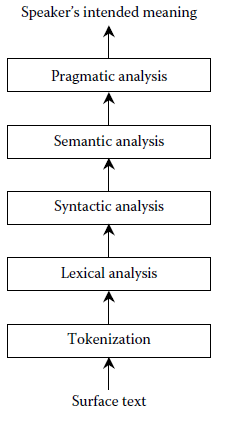
\includegraphics[width=7cm]{pictures/Analyseschritte.png}
\caption{Analyseschritte im klassischen NLP nach \cite[vgl.][4]{DALE}}
\label{fig:STEPS}
\end{wrapfigure}
\par
Den ersten Schritt bildet die \textit{Tokenization}. Zur Vorbereitung des Textes auf die weiteren Analyseschritte werden fundamentale Textbausteine, also Wörtern und Sätzen identifiziert. In segmentierten Sprachen wie dem Englischen, wird das \textit{White-Space-Zeichen} zum separieren der einzelnen Worte genutzt. Komplexe Probleme in diesem Zusammenhang sind beispielsweise die richtige Interpretation der Rolle eines Punktes (Satzende, Abkürzung oder Nummerntrennzeichen), der Umgang mit Mehrwortbenennungen oder die Normalisierung des Textes (Vereinheitlichung von unterschiedlicher Schreibweisen eines Wortes). Hierbei ist die Aussagekraft des Wort- oder Satzkontextes nicht zu unterschätzen. Für die Implementierung der Tokenization existieren zahlreiche regelbasierte Ansätze.
\par
Bei der lexikalischen Analyse wird der Text auf Ebene des einzelnen Wortes untersucht. Ein Wort bezeichnet hierbei eine Sammlung von Zeichenfolgen, die zu einem Lemma (Grundform) gehören. Im Rahmen der lexikalischen Analyse wird also einer Zeichenfolge (z.B. singt) ein Lemma mit Angaben zur Flexion (z.B. singen, 3. Person Singular Präsens) zugeordnet. Außerdem wird die Wortart (\textit{Part-Of Speech}) bestimmt. Im Vergleich zu anderen Sprachen, in denen durch Flexion zahlreiche komplexe Wortformen entstehen, ist diese Aufgabe im Englischen vergleichsweise einfach. Es stehen außerdem umfangreiche lexikale Ressourcen wie zum Beispiel das \textit{Princeton WordNet} für die lexikalische Analyse zur Verfügung. Andererseits entstehen hier erhebliche Schwierigkeiten bei der Identifizierung von Wortarten.
\par
Im Rahmen der syntaktische Analyse wird die Struktur eines Satzes analysiert. Zunächst wird die Satzart bestimmt. Den einzelnen Satzbausteinen wird dann ihre grammatikalische Funktion im Satz zugeordnet. Zusätzlich werden erste Abhängigkeiten identifiziert. Der eingesetzte \textit{Parser} ist im Idealfall effizient, robust und kann bei Mehrdeutigkeit die wahrscheinlichste Interpretation vorschlagen.
\par
Ziel der semantischen Analyse ist es, die Bedeutung des Textes zu erfassen. Der originale Text wird hierfür in eine Metasprache übersetzt. Basis hierfür ist die zuvor analysierte syntaktische Struktur der einzelnen Wörter und Sätze. Einige große Problem der semantischen Analyse sind der Umgang mit Mehrdeutigkeit, bildlicher Sprache und Ausdrücken, die aus mehreren Worten zusammengesetzt werden. Der Text wird deshalb in diesem Schritt um verschiedene Wortbedeutung mehrdeutiger Wörter, Wissensdomäne (Hyperonym), und Nomen-Pronomen Abhängigkeiten ergänzt (\textit{Coreference Resolution}). Alle extrahierten Informationen werden abschließend in einem \textit{Word Modell} zusammengetragen, das beispielsweise in einer objektorientierten Datenstruktur realisiert werden kann.

\par
Den abschließenden Schritt bildet die pragmatische Analyse. Hier wird entschieden, welche Reaktion aus den gewonnenen Informationen des World Modells abgeleitet werden soll. In der Regel wird ein weiterer Algorithmus mit Parametern versorgt und gestartet. Dieser beantwortet dann entweder eine Eingangsfrage, fasst den Text zusammen oder erstellt eine graphische Repräsenation des Textes wie beispielsweise ein Petri-Netz. Dieser Schritt wird im Rahmen dieser Seminararbeit jedoch nicht betrachtet.

Um einen gegebenen Text mit den genannten Annotationen anreichern zu können, sind spezielle Ressourcen und Tools nötig. Diese werden in Kapitel 2 ausführlich vorgestellt.







